% BIE = boundary integral equation. Build with latexmk main.tex.
\documentclass[review,hidelinks,onefignum,onetabnum]{siamart251216}

\usepackage{amsfonts,amssymb,mathtools,mathrsfs,bm,booktabs,xcolor}
\usepackage{tikz,pgfplots}
\pgfplotsset{compat=1.18}
\usepackage{amsopn}
\DeclareMathOperator{\diag}{diag}
\DeclareMathOperator{\ran}{ran}
\DeclareMathOperator{\ord}{ord}
\renewcommand{\Im}{\mathrm{Im}}
\renewcommand{\Re}{\mathrm{Re}}
\newcommand{\ii}{\mathrm{i}}
\newcommand{\ee}{\mathrm{e}}
\newcommand{\dd}{\mathrm{d}}
\newcommand{\CC}{\mathbb{C}}
\newcommand{\RR}{\mathbb{R}}
\newcommand{\ZZ}{\mathbb{Z}}
\newcommand{\QP}{\mathrm{QP}}
\newcommand{\rin}{\rho_{\min}}
\newcommand{\rax}{\rho_{\max}}
\newcommand{\creflastconjunction}{, and~}
\newsiamremark{remark}{Remark}
\newsiamremark{assumption}{Assumption}
\crefname{assumption}{Assumption}{Assumptions}
% Drafting note, printed in red; remove before submission.
\newcommand{\todo}[1]{\textcolor{red}{[TODO: #1]}}
\setlength{\emergencystretch}{1.5em}

\headers{A bordered Floquet closure for guided modes}{Author}
\title{Boundary integral computation of guided modes between periodic half-strips
  with a bordered Floquet closure\thanks{Submitted to the editors DATE.}}
\author{Author\thanks{Department of Mathematics, Example University, Example City
  (\email{author@example.com}).}}

\begin{document}
\maketitle

\begin{abstract}
A line defect between two periodic half-strips may support a guided mode at a
wavenumber where the Dirichlet-to-Neumann map of one half-strip has a pole.
The pole moves with the artificial vertical boundary and can obscure a zero
of the characteristic determinant. We construct a boundary integral solver
at fixed tangential Bloch wavenumber for piecewise constant media with
possibly different rods and periods on the two sides. A single-cell
scattering matrix gives the decaying Floquet subspace of each half-strip.
Matching these subspaces directly to the defect cell gives a bordered
matrix whose kernel is isomorphic to the discrete guided-mode space,
including at a singular Dirichlet trace. A determinant identity identifies
the factors introduced by Dirichlet elimination. A local analytic basis
permits interpolation of the bordered determinant on regular frequency
intervals. In an example with the rods held fixed, the bordered search
recovers the same mode as the artificial vertical boundary moves through
a position of numerical coincidence between the pole and the mode.
Unequal-period and published W3 waveguide examples test the solver on
different geometries. We report field jumps under refinement and compare
one guided wavenumber with independent finite element values.
\end{abstract}

% BIE = boundary integral equation.
\section{Introduction}\label{sec:intro}
Moving an artificial vertical boundary inside a homogeneous strip of a
photonic crystal leaves all rods in place. It can nevertheless move a pole
of the half-strip Dirichlet-to-Neumann (DtN) map directly onto a guided
wavenumber. A solver that locates zeros of a DtN determinant then faces two
distinct problems. An isolated pole can give a small ratio of extreme
singular values and pass a numerical acceptance test. If the pole and a
mode coincide, division by the singular Dirichlet trace can cancel the
zero itself. In the latter case even an exact evaluation of the reduced
determinant need not reveal the mode.

We consider a line defect between periodic dielectric half-strips. They
share the period along the defect and may differ in the transverse period,
rod shape and material. At fixed tangential Bloch wavenumber, an eigenvalue
in a common gap of the surrounding crystals has a field decaying into
both half-strips \cite{Fliss2013,KlindworthSchmidtFliss2014}. Our aim is to
compute such wavenumbers and fields by discretizing the material interfaces.
The method uses a boundary integral equation (BIE) for the response of a
cell, Rayleigh amplitudes to exchange fields between adjacent cells, and
Floquet modes to represent decay at infinity.

\paragraph{Transparent boundaries and existing solvers}
Cell-based transparent conditions reduce the unbounded problem to the
defect region \cite{JolyLiFliss2006,Fliss2013}.
Klindworth, Schmidt and Fliss \cite{KlindworthSchmidtFliss2014} treated
different periodic claddings by finite elements. Fliss, Klindworth and
Schmidt \cite{FlissKlindworthSchmidt2015} distinguished global half-strip
Dirichlet exceptional values from local cell exceptional values. Their
Robin-to-Robin (RtR) formulation handles these values through Robin data.
It provides a natural comparison for a method that already has access to
both components of the trace. In the present formulation the full
half-strip data are available directly from the decaying Floquet subspace.
We retain its coefficients and impose membership in that subspace on each
side of the defect.

\paragraph{Scattering matrices and boundary integral determinants}
Gralak, Enoch and Tayeb \cite{GralakEnochTayeb2002} compute Bloch modes
from a layer scattering matrix. Botten et al.\ \cite[eq.~(38)]{BottenEtAl2004}
write continuity at an interface between two photonic crystals as equality
of the complete plane-wave states expanded in the two Bloch bases. They
subsequently derived a determinant equation for defect modes in cylinder
arrays \cite{BottenEtAl2006}. Their W3 guide supplies an external benchmark
below. In a BIE for forced scattering by periodic layers, Cho and Barnett
\cite[eqs.~(47) and~(53)]{ChoBarnett2015} retain the outgoing Rayleigh
amplitudes together with the layer densities and match the field and its
normal derivative. Here the exterior states are the decaying Floquet
subspaces of periodic half-strips.
Barnett and Greengard \cite{BarnettGreengard2010} showed how a change of
integral representation avoids empty-cell resonances in a doubly periodic
band-structure calculation. Zhao and Barnett \cite{ZhaoBarnett2015} used an
analytic Fredholm determinant and polynomial interpolation to compute
Dirichlet eigenvalues of a bounded domain. Here the representation
singularity arises when the decaying half-strip data are written as a graph
over their Dirichlet traces. For a direct subspace determinant, orthonormal bases returned by independent
generalized Schur decompositions need not vary continuously with frequency.

\paragraph{The discrete guided-mode problem}
We apply direct modal matching to the defect-cell BIE and the two decaying
Floquet subspaces. We prove the dimension count for the flux-conserving
truncated cell and identify the kernel of the resulting bordered matrix.
For this discretization, block elimination gives the precise relation
between the full matching determinant and the DtN determinant. The factors include the center density block, both Dirichlet
trace blocks and the Rayleigh-to-Cauchy coordinate changes. Their orders
explain when Dirichlet elimination can obscure a mode in this solver.
A locally normalized basis then yields an analytic
determinant wherever the cell assembly and the subspace separation are
regular. The same trace data also give the discrete RtR formulation.

To test the mechanism we compute the same waveguide with the artificial
vertical boundary in three positions. One position puts a Dirichlet pole
near the mode and another aligns them to numerical precision. We compare
the returned frequencies, the status of the whole search window and jumps
of the reconstructed fields. An empty defect between unequal-period
half-strips, the W3 guide and a finite element refinement provide separate
checks. The mathematical kernel statements concern the discrete matching
equations. The experiments assess how their roots approximate physical
wavenumbers.

\Cref{sec:model} defines the waveguide and the frequency window.
\Cref{sec:discretization,sec:leads} construct the cell data and the decaying
spaces. \Cref{sec:closure} derives the bordered determinant and its relation
to the DtN and RtR descriptions. \Cref{sec:algorithm,sec:experiments}
describe the search, field reconstruction and numerical tests.

% Section 2: model problem, the computational task, and the two kinds of
% representation singularity. Cell notation follows draft/bie-siam Section 2.1.
\section{Model problem and computational task}\label{sec:model}

\subsection{Periodic media with a line defect}\label{sec:geometry}
For $s\in\{-,+\}$ let $\rho_s$ be a coefficient with periods $L_s>0$ in $x$ and
$d>0$ in $y$. The two sides share the period $d$; $L_-$ and $L_+$ may differ.
Each $\rho_s$ is piecewise constant. In a common background value
$\rho_{\mathrm e}>0$, every period cell of $\rho_s$ contains finitely many
simply connected rods with $C^2$ boundaries and constant values. The
coefficient $\rho$ of the waveguide equals $\rho_-$ for $x<x_-$ and $\rho_+$
for $x>x_+$. The \emph{defect cell} $(x_-,x_+)\times I_d$, with $x_\pm=\pm L_0/2$ and
$I_d:=(-d/2,d/2)$, contains one further rod $\Omega_0$ or none. All rod
closures stay away from the cell boundaries. We write
$0<\rin\le\rho\le\rax$ and $B:=\RR\times I_d$. The two \emph{periodic
half-strips} are $S_-=(-\infty,x_-)\times I_d$ and $S_+=(x_+,\infty)\times I_d$, with
coefficients $\rho_-$ and $\rho_+$; \cref{fig:model-geometry} shows the geometry.

The defect cell and the $j$th periodicity cells of $S_+$ and $S_-$ ($j\ge0$) are
\[
\begin{gathered}
  \mathcal C_0=(x_-,x_+)\times I_d,\qquad
  \mathcal C_{j,+}=(x_++jL_+,\,x_++(j+1)L_+)\times I_d,\\
  \mathcal C_{j,-}=(x_--(j+1)L_-,\,x_--jL_-)\times I_d .
\end{gathered}
\]
The vertical lines $\{x_\pm\}\times I_d$ are the \emph{artificial (vertical)
boundaries} of the defect cell; the lines between consecutive periodicity
cells are
the \emph{walls}. Every artificial boundary and every wall lies in a vertical
strip of pure background between two groups of rods. We call the largest such
open strip containing a given line its \emph{gap strip}, and its width $w$ the
gap width; $w_{\min}$ denotes the smallest gap width over all artificial
boundaries and walls. The position of these lines inside their gap strips is
a free parameter of the computation. When we speak of \emph{moving an
artificial boundary}, we mean moving this line inside its gap strip, which
changes no physical quantity.

% Geometry of the two periodic half-strips and the line defect in Section 2.1.
\begin{figure}[htbp]
\centering
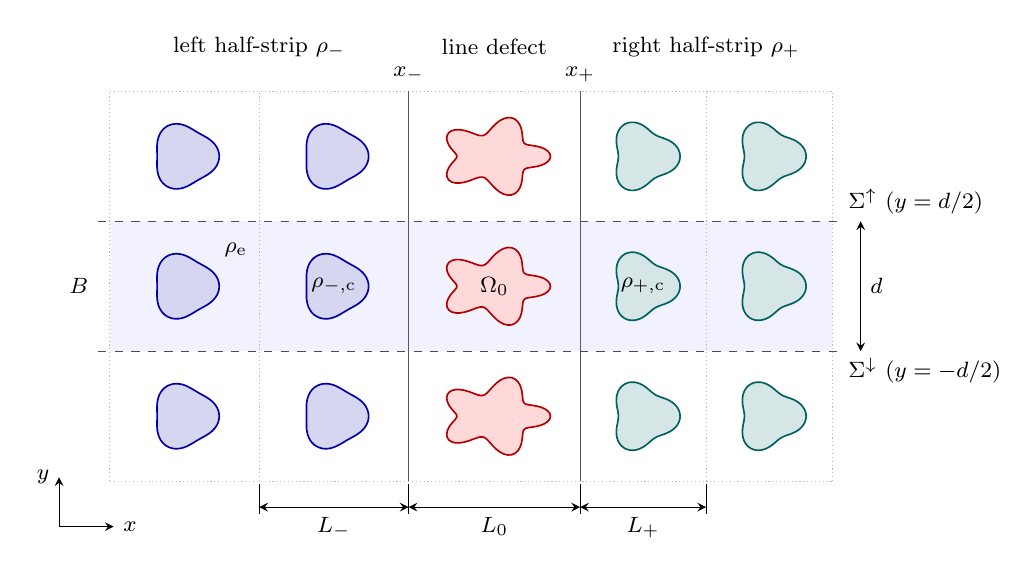
\begin{tikzpicture}[x=1.65cm,y=1.65cm,font=\footnotesize,>=stealth,
  cell wall/.style={gray!55,densely dotted,thin},
  seam/.style={black!70,dashed,thin},
  measure/.style={<->,thin},
  pics/lead rod/.style args={#1/#2}{code={
    \filldraw[draw=#1,fill=#1!16,line width=.6pt]
      plot[domain=0:360,samples=73,variable=\t]
      ({.24*(1+#2*cos(3*\t))*cos(\t)/sqrt(1+#2*#2/2)},
       {.24*(1+#2*cos(3*\t))*sin(\t)/sqrt(1+#2*#2/2)}) -- cycle;}},
  pics/defect rod/.style={code={
    \filldraw[draw=red!70!black,fill=red!15,line width=.6pt]
      plot[domain=0:360,samples=91,variable=\t]
      ({.24*(1.5+.3*cos(5*\t))*cos(\t)},
       {.24*(1+.3*cos(5*\t))*sin(\t)}) -- cycle;}}]
  % Two full periodicity cells on each side; three transverse periods.
  \fill[blue!5] (-2.96,-.5) rectangle (2.60,.5);
  \foreach \x in {-2.96,-1.81,1.63,2.60}
    \draw[cell wall] (\x,-1.5) -- (\x,1.5);
  \foreach \y in {-1.5,1.5}
    \draw[cell wall] (-2.96,\y) -- (2.60,\y);
  \foreach \x in {-.66,.66}
    \draw[black!65,thin] (\x,-1.5) -- (\x,1.5);
  \foreach \y in {-.5,.5}
    \draw[seam] (-3.05,\y) -- (2.69,\y);
  \foreach \y in {-1,0,1} {
    \foreach \x in {-2.385,-1.235}
      \pic at (\x,\y) {lead rod={blue!65!black/.12}};
    \pic at (0,\y) {defect rod};
    \foreach \x in {1.145,2.115}
      \pic at (\x,\y) {lead rod={teal!75!black/.20}};
  }
  \node at (-1.81,1.84) {left half-strip $\rho_-$};
  \node at (0,1.84) {line defect};
  \node at (1.63,1.84) {right half-strip $\rho_+$};
  \node[above] at (-.66,1.5) {$x_-$};
  \node[above] at (.66,1.5) {$x_+$};
  \node at (0,0) {$\Omega_0$};
  \node at (-1.99,.28) {$\rho_{\mathrm e}$};
  \node at (-1.235,0) {$\rho_{-,\mathrm c}$};
  \node at (1.145,0) {$\rho_{+,\mathrm c}$};
  \node[left] at (-3.05,0) {$B$};
  \draw[measure] (2.82,-.5) -- node[right] {$d$} (2.82,.5);
  \node[above right,inner sep=1pt] at (2.70,.53)
    {$\Sigma^\uparrow\ (y=d/2)$};
  \node[below right,inner sep=1pt] at (2.70,-.53)
    {$\Sigma^\downarrow\ (y=-d/2)$};
  \foreach \a/\b/\period in {-1.81/-.66/L_-,-.66/.66/L_0,.66/1.63/L_+} {
    \draw[thin] (\a,-1.52) -- (\a,-1.75);
    \draw[measure] (\a,-1.70) -- node[below] {$\period$} (\b,-1.70);
  }
  \draw[thin] (1.63,-1.52) -- (1.63,-1.75);
  \draw[->] (-3.35,-1.85) -- ++(.42,0) node[right] {$x$};
  \draw[->] (-3.35,-1.85) -- ++(0,.38) node[left] {$y$};
\end{tikzpicture}
\caption{Two periodic half-strips separated by a line defect with defect rod
$\Omega_0$. The solid vertical lines at $x_\pm$ are the artificial vertical boundaries; dotted vertical lines are periodicity-cell walls. The shaded row is one period
strip $B=\RR\times I_d$; translation from its lower edge to its upper edge
multiplies the field by $\ee^{\ii\beta d}$.}
\label{fig:model-geometry}
\end{figure}


Fix $\beta\in[-\pi/d,\pi/d)$. A \emph{guided mode} at wavenumber $k>0$ is a
nonzero solution of $-\Delta w=k^2\rho w$ in $\RR^2$ of the form
$w=v\,\ee^{\ii\beta y}$ with $v$ $d$-periodic in $y$ and $v|_B\in H^1(B)$
\cite{Fliss2013}. The value and the normal derivative of $w$ are continuous
across every rod boundary. Equivalently, $k^2$ is an eigenvalue of the
nonnegative self-adjoint operator $A(\beta)=-\rho^{-1}\Delta$ in
$L^2(B,\rho\,\dd x\,\dd y)$ with $\ee^{\ii\beta d}$-quasi-periodic conditions on
the upper and lower edges of $B$ \cite[sect.~3]{Fliss2013}. Its essential
spectrum is the union of the spectra of the two periodic operators $A_\pm(\beta)$
obtained by extending $\rho_\pm$ to the whole strip
\cite[Prop.~2.1]{KlindworthSchmidtFliss2014}. Each of these is a union of
bands over the Bloch wavenumber along $x$ \cite{Kuchment1993}. An
open interval disjoint from both spectra is a \emph{common gap}
$G_\beta$. Guided modes with $k^2\in G_\beta$ are isolated eigenvalues of
finite multiplicity, and their fields decay exponentially into both half-strips.

\subsection{Rayleigh orders and Wood points}\label{sec:rayleigh}
Let $\beta_m=\beta+2\pi m/d$ and $\psi_m(y)=d^{-1/2}\ee^{\ii\beta_my}$, an
orthonormal basis of $\beta$-quasi-periodic functions on $I_d$. With
$\kappa_{\mathrm e}=k\rho_{\mathrm e}^{1/2}$ the background wavenumber, the
$m$th Rayleigh order has the normal wavenumber
\begin{equation}\label{eq:gamma}
  \gamma_m(k)=\bigl(\kappa_{\mathrm e}^2-\beta_m^2\bigr)^{1/2},\qquad
  \gamma_m>0\ \text{or}\ \Im\gamma_m>0 .
\end{equation}
The order is \emph{propagating} if $\gamma_m>0$ and \emph{evanescent} if
$\gamma_m=\ii\kappa_m$ with $\kappa_m>0$. A \emph{Wood point} is a wavenumber
with $\gamma_m(k)=0$ for some $m$, that is, $\kappa_{\mathrm e}=|\beta_m|$. In
the examples of \cref{sec:experiments} the line $k=|\beta|$ ($m=0$,
$\rho_{\mathrm e}=1$) crosses the common gap, and guided branches cross it.
At a Wood point the guided-mode problem itself is regular: nothing in the
definition above refers to the Rayleigh orders of the background.

\subsection{The computational task}\label{sec:task}
\begin{quote}
\textbf{Task.} Given the geometry, the coefficients, $\beta$ and a window
$[k_1,k_2]$ with $[k_1^2,k_2^2]\subset G_\beta$, return all guided-mode
wavenumbers in the window, with their fields.
\end{quote}
We ask a solver for this task to meet five requirements.
\begin{enumerate}
\item No root is returned that is not a guided mode of the discretized problem.
\item No guided mode in the window is missed.
\item The returned wavenumbers are accurate to near machine precision when the
  discretization is refined.
\item The result does not depend on the arbitrary choices of the computation:
  the position of the artificial boundaries and walls inside their gap
  strips, the Rayleigh
  truncation $M$ beyond its convergence threshold, and the basis of any
  subspace.
\item Where an assumption of the method fails, the solver says so instead of
  returning a wrong answer.
\end{enumerate}

A method reduces the task to the zeros of a characteristic function of $k$,
here a determinant. We call a wavenumber in the window a
\emph{representation singularity} if the guided-mode problem is regular
there, but the characteristic function is singular or undefined, or vanishes
without a guided mode. Such points break requirement 1, 2 or 4, depending on
where they fall. Fliss, Klindworth and Schmidt observed two kinds for the
Dirichlet-to-Neumann closure of a finite element method
\cite{FlissKlindworthSchmidt2015}: global ones, where the Dirichlet problem in
a half-strip is not uniquely solvable, and local ones, where the Dirichlet
problem in one cell is not uniquely solvable; they removed both with
Robin-to-Robin maps. The boundary integral method of this paper has the
following two kinds.
\begin{itemize}
\item \emph{Global: Dirichlet exceptional values of the closure.} These
  are wavenumbers at which a decaying half-strip solution vanishes on the
  artificial boundary, in the retained orders. They move when the artificial
  boundary is moved.
  \Cref{sec:closure} shows how they enter the determinant and removes them.
\item \emph{Local: singularities of the cell scattering problem.} Each cell
  is solved as a single row of rods, repeated in $y$, in an infinite
  background with outgoing Rayleigh conditions. This fails in two ways.
  First, at Wood points the amplitude coordinates on the artificial boundaries
  and walls degenerate
  and the extraction formulas contain $1/\gamma_m$. Second, the row alone may
  carry a trapped mode at $(\beta,k)$, in which case the cell scattering
  problem is not uniquely solvable. The second case is the analogue of the
  local Dirichlet values of \cite{FlissKlindworthSchmidt2015}. We did not
  observe it in our examples, and the solver monitors the conditioning of
  every cell solve. The solver does not remove the Wood singularity;
  \cref{sec:wood} explains it and describes how the search avoids it.
\end{itemize}

% Method section of the solver paper. Moved verbatim from draft/bie-siam
% (Section 3, commit cc23eea) on 2026-11-07; to be rewritten (see README.md).
\section{Discretization and candidate computation}\label{sec:discretization}

Candidates are computed on the center cell, as in the transparent boundary
conditions of Fliss \cite[Thm.~4.5]{Fliss2013}: a guided mode restricted to
$\mathcal C_0$ has port Cauchy data of finite-energy half-guide solutions. The
Dirichlet-to-Neumann form of this condition fails at countably many Dirichlet
eigenvalues in the gap \cite[Thm.~4.1]{Fliss2013}, which Robin-to-Robin
conditions avoid \cite{FlissKlindworthSchmidt2015}; we impose instead that the
port states lie in the decaying subspaces themselves. Lead cells are
discretized by boundary integral equations with port Rayleigh amplitudes, the
decaying half-guide solutions by an ordered QZ decomposition, and the center
cell by layer potentials plus background Rayleigh waves. The output is a
candidate $\widehat k$ with coefficients. We make no claim on its accuracy here:
the enclosure paper~\companion bounds the spectral distance of whatever field these
coefficients define. Fix $\beta$ and a wavenumber $k>0$ with $k^2\in G_\beta$.

\subsection{Port Fourier basis and Rayleigh waves}
Let $\beta_m=\beta+2\pi m/d$, $\psi_m(y)=d^{-1/2}\ee^{\ii\beta_my}$, truncated to
$|m|\le M$, $K=2M+1$. With $\kappa_{\mathrm e}=k\rho_{\mathrm e}^{1/2}$ let
$\gamma_m=(\kappa_{\mathrm e}^2-\beta_m^2)^{1/2}$ with $\Im\gamma_m\ge0$, and
$\boldsymbol\gamma=\diag(\gamma_m)$. We assume that $k$ is not a Wood point,
that is, $\gamma_m(k)\ne0$ for all $m\in\ZZ$. Only the candidate search uses
this; the bound of the enclosure paper~\companion does not.

In a vertical background strip, a $\beta$-quasi-periodic Helmholtz solution is
$u=\sum_m(a_mr_m^{x_p}+b_ml_m^{x_p})$ with
$r_m^{x_p}=\ee^{\ii\gamma_m(x-x_p)}\psi_m$ and
$l_m^{x_p}=\ee^{-\ii\gamma_m(x-x_p)}\psi_m$; $(a,b)$ are the right- and
left-going amplitudes anchored at $x_p$. Moving the anchor by $\ell$ multiplies
amplitudes by $\mathsf E(\ell)=\diag(\ee^{\ii\gamma_m\ell})$. For a port with
normal $\pm e_x$, amplitudes map to the Fourier coefficients of (value, normal
derivative) by $\mathsf C_\pm=\left[\begin{smallmatrix}I&I\\
\pm\ii\boldsymbol\gamma&\mp\ii\boldsymbol\gamma\end{smallmatrix}\right]$,
invertible away from Wood points.

\subsection{Layer potentials on a rod}\label{sec:layer}
Let $G^{(\kappa)}$ be the free-space Green function $\frac{\ii}{4}H^{(1)}_0(\kappa|
\mathbf z-\mathbf z'|)$ and $G^{(\kappa)}_\QP$ the $\ee^{\ii\beta d}$-quasi-periodic
one. We use the near-image split
\begin{equation}\label{eq:near-image}
  G^{(\kappa)}_\QP(\mathbf z,\mathbf z')=\sum_{n=-1}^{1}\ee^{\ii\beta nd}G^{(\kappa)}(\mathbf z,
  \mathbf z'+nd\,e_y)+G^{(\kappa)}_{\mathrm{far}}(\mathbf z-\mathbf z'),
\end{equation}
where $G^{(\kappa)}_{\mathrm{far}}$ is a smooth Helmholtz solution away from the
images $|n|\ge2$, since $(\Delta+\kappa^2)G^{(\kappa)}_\QP(\cdot,\mathbf 0)=
-\sum_n\ee^{\ii\beta nd}\delta_{nd\,e_y}$ \cite{Linton1998}. For a curve strictly inside a cell,
a quasi-periodic layer potential is thus three free-space layer potentials plus
a smooth correction near the closed cell, the structure used in
\cite{BarnettGreengard2010,BarnettGreengard2011,ChoBarnett2015}; the smooth
correction and the background are represented together by proxy point sources
outside the cell, with coefficients fitted to the quasi-periodicity on the top
and bottom seams. Since the enclosure paper~\companion checks only the jumps of an explicit
field, the densities may be computed with any adequate approximation of
$G_\QP$; the field evaluated in the enclosure paper~\companion uses the split
\eqref{eq:near-image} and fixed proxies, and all its mismatch enters its own
jumps.

For a rod $\Omega$ with $C^2$ boundary, outward normal $\nu$, and interior
wavenumber $\kappa_{\mathrm c}=k\rho_{\mathrm c}^{1/2}$, we represent the field in
the cell by
\begin{equation}\label{eq:cell-rep}
  u=\mathcal S^{(\kappa_{\mathrm e})}_\QP[\omega]+\mathcal D^{(\kappa_{\mathrm e})}_\QP[\tau]
  +u_{\mathrm b}\ \text{outside }\Omega,\qquad
  u=\mathcal S^{(\kappa_{\mathrm c})}[\omega]+\mathcal D^{(\kappa_{\mathrm c})}[\tau]
  \ \text{in }\Omega,
\end{equation}
with a finite background Rayleigh field $u_{\mathrm b}$. By the jump relations
\cite{ColtonKress1983,Kress1991}, the outside-minus-inside jumps of value and
normal derivative are, with $\eta=(\tau;-\omega)$,
\begin{equation}\label{eq:jump-operator}
  \mathscr J_k[\eta;u_{\mathrm b}]=
  \begin{bmatrix}
    I+D^{(\kappa_{\mathrm e})}_\QP-D^{(\kappa_{\mathrm c})}&-S^{(\kappa_{\mathrm e})}_\QP+S^{(\kappa_{\mathrm c})}\\
    T^{(\kappa_{\mathrm e})}_\QP-T^{(\kappa_{\mathrm c})}&I-D'^{(\kappa_{\mathrm e})}_\QP+D'^{(\kappa_{\mathrm c})}
  \end{bmatrix}\eta
  +\begin{bmatrix}u_{\mathrm b}\\ \partial_\nu u_{\mathrm b}\end{bmatrix}_{\partial\Omega}.
\end{equation}
The transmission conditions are $\mathscr J_k=0$, a second-kind system in which
the hypersingular parts cancel \cite{DominguezLyonTurc2016}. We discretize it by
Nystr\"om quadrature with Kress's logarithmic splitting on a uniform parameter
grid \cite{Kress1991,HaoBarnettMartinssonYoung2014}; $n$ is the number of density
unknowns. By the spectral representation of $G_\QP$, the potentials of a curve
lying left (right) of a line $x=x_p$ are purely right- (left-) going there;
their amplitudes are integrals of $\omega$ and $\tau$ against explicit
exponentials, and quadrature gives extraction matrices
$\mathsf F^{\rightarrow}_{x_p},\mathsf F^{\leftarrow}_{x_p}\in\CC^{K\times n}$.

\subsection{Lead cells: scattering matrix and decaying subspace}\label{sec:lead}
In the right cell $\mathcal C_{0,+}$ with ports $x_{\mathrm L}=x_+$,
$x_{\mathrm R}=x_++L_+$, the incident field
$u_{\mathrm b}=\sum_m(a_{\mathrm L,m}r_m^{x_{\mathrm L}}+b_{\mathrm R,m}l_m^{x_{\mathrm R}})$
determines $\eta$ through $\mathscr J_k[\eta;u_{\mathrm b}]=0$, and the outgoing
amplitudes are $b_{\mathrm L}=\mathsf E(L_+)b_{\mathrm R}+\mathsf F^{\leftarrow}_{x_{\mathrm L}}\eta$,
$a_{\mathrm R}=\mathsf E(L_+)a_{\mathrm L}+\mathsf F^{\rightarrow}_{x_{\mathrm R}}\eta$.
This defines the cell scattering matrix
$[b_{\mathrm L};a_{\mathrm R}]=[R_{\mathrm L},T_{\mathrm{RL}};T_{\mathrm{LR}},R_{\mathrm R}]
[a_{\mathrm L};b_{\mathrm R}]$, or equivalently, for the port states
$z_{\mathrm L}=(a_{\mathrm L};b_{\mathrm L})$ and $z_{\mathrm R}=(a_{\mathrm R};b_{\mathrm R})$,
\begin{equation}\label{eq:pencil}
  \mathsf E_{\mathrm L}z_{\mathrm L}=\mathsf E_{\mathrm R}z_{\mathrm R},\qquad
  \mathsf E_{\mathrm L}=\begin{bmatrix}-R_{\mathrm L}&I\\T_{\mathrm{LR}}&0\end{bmatrix},\quad
  \mathsf E_{\mathrm R}=\begin{bmatrix}0&T_{\mathrm{RL}}\\I&-R_{\mathrm R}\end{bmatrix}.
\end{equation}
The left cell, with its own rod, contrast and width $L_-$, is treated in the
same way. Floquet solutions satisfy $\mathsf E_{\mathrm L}z=\zeta\mathsf E_{\mathrm R}z$
with multiplier $\zeta=\ee^{\ii\theta L_+}$. In a gap the continuous
multipliers pair as $\zeta\leftrightarrow1/\bar\zeta$; the pairing
$\zeta\leftrightarrow1/\zeta$ of \cite{JolyLiFliss2006} corresponds to
replacing $\beta$ by $-\beta$ and agrees with the fixed-$\beta$ problem only
under $y\mapsto-y$ symmetry. Neither implies that the discrete pencil has
exactly $K$ multipliers inside the unit circle, so this is checked.

An ordered QZ decomposition $\mathsf Q\mathsf E_{\mathrm L}\mathsf Z=\mathsf U_{\mathrm L}$,
$\mathsf Q\mathsf E_{\mathrm R}\mathsf Z=\mathsf U_{\mathrm R}$ with the $K$
eigenvalues $|\zeta|<1$ first gives the leading columns $\mathsf Z_+$ and
\begin{equation}\label{eq:propagation}
  \mathsf P_+=\mathsf U_{\mathrm R,11}^{-1}\mathsf U_{\mathrm L,11},\qquad
  \mathsf E_{\mathrm L}\mathsf Z_+=\mathsf E_{\mathrm R}\mathsf Z_+\mathsf P_+ .
\end{equation}
Hence the port states $z_j=\mathsf Z_+\mathsf P_+^jc$ of consecutive cells are
compatible and decay geometrically: the discrete analogue of the
finite-energy solutions in the right half guide. On the left, the $K$ eigenvalues $1/\zeta$ inside the unit circle of the pencil
$(\mathsf E_{\mathrm R},\mathsf E_{\mathrm L})$ give $\mathsf Z_-$ and $\mathsf P_-$ with
$\mathsf E_{\mathrm R}\mathsf Z_-=\mathsf E_{\mathrm L}\mathsf Z_-\mathsf P_-$.
Using the whole Schur subspace keeps multiple and nonnormal multipliers; a
change of basis $\mathsf Z_\pm\mapsto\mathsf Z_\pm W$ only conjugates
$\mathsf P_\pm$. If the pencil is singular, the cluster dimension is not $K$,
or the cluster is not separated from the unit circle, the discretization at
that $k$ is rejected. The discrete Cauchy data spaces are
$\mathcal G^h_\pm(k)=\operatorname{range}\mathsf C_\pm\mathsf Z_\pm$.

\subsection{Center cell}\label{sec:center}
In $\mathcal C_0$ we use \eqref{eq:cell-rep} with $\Omega=\Omega_0$ (no layer
potentials if $\Omega_0=\varnothing$) and
\[
  u_{\mathrm b}=u_{\mathrm{hom}}=\sum_m\bigl(a^-_{0,m}r_m^{x_-}+b^+_{0,m}l_m^{x_+}\bigr),
\]
the part of the field entering through the two ports. It may be nonzero even
if $\Omega_0=\varnothing$, so quasi-periodic layer potentials alone do not
represent the center field. The ansatz follows the complementary-field
representation of \cite[App.~A]{BarnettGreengard2010} with the incident port
terms added. We use it only as an ansatz; neither completeness nor uniqueness of
the representation enters the enclosure paper~\companion.

After truncation, the center unknown is $\xi=(\eta;a^-_0;b^+_0)\in\CC^{n+2K}$
($n=0$ for an empty center), and the discrete transmission equations read
$J(k)\xi=0$. The center field has the port amplitudes
\[
  \mathsf Y_-\xi=\begin{bmatrix}a^-_0\\ \mathsf F^{\leftarrow}_{x_-}\eta+\mathsf E(L_0)b^+_0\end{bmatrix},
  \qquad
  \mathsf Y_+\xi=\begin{bmatrix}\mathsf F^{\rightarrow}_{x_+}\eta+\mathsf E(L_0)a^-_0\\ b^+_0\end{bmatrix}.
\]

\subsection{Discrete eigenvalue problem and candidates}\label{sec:nep}
A candidate is a center solution whose port states lie in the decaying
subspaces: we ask for $\xi\ne0$ and $c_\pm\in\CC^K$ with
\begin{equation}\label{eq:nep}
  J(k)\xi=0,\qquad \mathsf Y_\pm\xi=\mathsf Z_\pm c_\pm .
\end{equation}
For root finding we need a scalar function that is analytic in $k$ and
independent of the basis of the stable subspaces; the determinant of the full
system \eqref{eq:nep} is neither. We therefore eliminate the center densities,
treat the center as a scattering cell with incident port amplitudes $\mathsf a\in\CC^{2K}$,
and let $\mathsf T_0(k)$, $\mathsf N_0(k)$ map $\mathsf a$ to the value and
normal-derivative coefficients of the total field at both ports. With the value
and normal-derivative blocks $\mathsf C_\pm\mathsf Z_\pm=[\mathsf D_\pm;\mathsf N_\pm]$
of the stable subspaces, the discrete DtN matrices are
$\Lambda_\pm=\mathsf N_\pm\mathsf D_\pm^{-1}$, and
\begin{equation}\label{eq:port-matrix}
  \mathsf A(k)=\mathsf N_0(k)-\diag\bigl(\Lambda_-(k),\Lambda_+(k)\bigr)\mathsf T_0(k)
  \in\CC^{2K\times2K}.
\end{equation}
On a complex neighborhood of a real interval free of Wood points, if both pencils
are regular with the stable cluster separated from the rest, and the matrices
used in the elimination are invertible, then $\det\mathsf A$ is analytic except
for poles where $\mathsf D_\pm$ or those matrices are singular. A singular
$\mathsf D_\pm$ is the discrete counterpart of a Dirichlet exceptional value
\cite[Thm.~4.1]{Fliss2013}, at which \eqref{eq:nep} remains valid. These conditions are monitored only at
interpolation nodes; they are empirical checks of the search, on which the final
interval does not depend.

\emph{Root search.} On each piece of the gap we interpolate $f(k)=\det\mathsf A(k)$
(computed by LU, as log-modulus and phase) at nested Chebyshev--Lobatto nodes of
degree $4,8,\dots,64$ until the trailing coefficients fall below $10^{-10}$ and two
off-grid checks agree to $10^{-9}$, bisecting otherwise; roots of the interpolant
come from the colleague matrix and are polished by Newton steps on the
interpolant \cite{Boyd2002,ZhaoBarnett2015}. A root is accepted if the scaled
singular-value ratio $s(\widehat k)=\sigma_{\min}/\sigma_{\max}$ of
$W_r\mathsf A(\widehat k)W_c$ is below $10^{-11}$; failures fall back to bisection
on $s(k)$. The candidate output is the right singular vector of the smallest
singular value, which determines $\mathsf a$, the center densities, and the lead
coordinates $c_\pm$. Together with $\widehat k$, $\mathsf P_\pm$, $\mathsf Z_\pm$
and the discretization parameters, these are the only inputs of
the enclosure paper~\companion. A small $s(\widehat k)$ says that a finite system is nearly
singular, not how far $\widehat k^2$ is from $\sigma(A(\beta))$.

% Section 4: Floquet eigenvalue problem of a periodicity cell, flux identity, dimension of the decaying subspaces
% (Lemma A of research/projects/bie-enclosure/theory/port-subspace.md, reviewed
% 12/12 in port-subspace-review.md), the fully discrete criterion, ordered QZ.
\section{Decaying subspaces of the half-strips}\label{sec:leads}

\subsection{The Floquet eigenvalue problem}\label{sec:pencil}
Anchor the port states of one periodicity cell at its own walls,
$z_{\mathrm L}=(a_{\mathrm L};b_{\mathrm L})$ and $z_{\mathrm R}=(a_{\mathrm R};b_{\mathrm R})$.
The scattering relation \eqref{eq:smatrix} is equivalent to
\begin{equation}\label{eq:pencil}
  \mathsf E_{\mathrm L}z_{\mathrm L}=\mathsf E_{\mathrm R}z_{\mathrm R},\qquad
  \mathsf E_{\mathrm L}=\begin{bmatrix}-R_{\mathrm L}&I\\ T_{\mathrm{LR}}&0\end{bmatrix},\qquad
  \mathsf E_{\mathrm R}=\begin{bmatrix}0&T_{\mathrm{RL}}\\ I&-R_{\mathrm R}\end{bmatrix}.
\end{equation}
In a periodic half-strip the right wall of one cell is the left wall of the
next.
A sequence of states $(z_j)_{j\ge0}$ on consecutive walls is compatible if
$\mathsf E_{\mathrm L}z_j=\mathsf E_{\mathrm R}z_{j+1}$ for all $j$. A Floquet
solution $z_{j+1}=\zeta z_j$ solves the \emph{Floquet eigenvalue problem}
\begin{equation}\label{eq:floquet}
  (\mathsf E_{\mathrm L}-\zeta\mathsf E_{\mathrm R})\,z_0=0,
\end{equation}
a generalized eigenvalue problem whose eigenvalue $\zeta$ is the Floquet
multiplier of the solution (in numerical linear algebra,
$\mathsf E_{\mathrm L}-\zeta\mathsf E_{\mathrm R}$ is the matrix pencil
$(\mathsf E_{\mathrm L},\mathsf E_{\mathrm R})$). We call the problem \emph{regular} if
$\det(\mathsf E_{\mathrm L}-\zeta\mathsf E_{\mathrm R})$ does not vanish identically in
$\zeta$. It then has $2K$ multipliers in $\CC\cup\{\infty\}$, counted with
algebraic multiplicity; $\zeta=\infty$ occurs when $\mathsf E_{\mathrm R}$ is singular. For $S_+$ we need the subspace of initial states whose
compatible sequences are square summable, and for $S_-$ the
analogous subspace towards $-\infty$, obtained from the reversed problem
$(\mathsf E_{\mathrm R}-\zeta\mathsf E_{\mathrm L})z_0=0$.

The continuous half-strip has as many decaying as growing solutions in a
gap. For the discrete problem this count is not automatic. A $2K\times2K$
generalized eigenvalue problem may have any number of multipliers inside the unit circle, and if the number is
not $K$, the closure of \cref{sec:closure} is not square. The next lemma
shows that the count follows from energy conservation of the truncated cell.

\subsection{Flux and the dimension of the decaying subspace}\label{sec:flux}
Let $u_M$ be the retained part \eqref{eq:rayleigh} of a field on a wall. Its
flux through the wall in the direction $+e_x$ is a Hermitian form in the
port state:
\begin{equation}\label{eq:flux}
  \Phi(z)=\Im\int_{I_d}\overline{u_M}\,\partial_xu_M\,\dd y=z^*\mathsf J z,
  \qquad
  \mathsf J=\begin{bmatrix}\Re\boldsymbol\gamma&-\ii\Im\boldsymbol\gamma\\
     \ii\Im\boldsymbol\gamma&-\Re\boldsymbol\gamma\end{bmatrix}.
\end{equation}
Indeed, the cross terms between different orders vanish by orthogonality. A
propagating order contributes $\gamma_m(|a_m|^2-|b_m|^2)$, and an evanescent
order contributes $2\kappa_m\Im(\bar a_mb_m)$. Each $2\times2$ block of
$\mathsf J$ has eigenvalues $\pm|\gamma_m|$. Away from Wood points
$\mathsf J$ is therefore nondegenerate with $K$ positive and $K$ negative
eigenvalues.

\begin{assumption}[truncated periodicity cell]\label{ass:cell}
$k>0$ and $\beta$ are real, every propagating order is retained, and no
retained order is at a Wood point. The scattering matrix in
\eqref{eq:pencil} is that of the exact single-cell problem: retained incident
orders, zero incident amplitude in the deleted orders, and outgoing fields in
all orders. This problem has a unique solution for every incident vector.
\end{assumption}

\begin{lemma}[dimension of the decaying subspaces]\label{lem:dimension}
Under \cref{ass:cell}, suppose the problem \eqref{eq:floquet} is regular and
$\mathsf E_{\mathrm L}-\zeta\mathsf E_{\mathrm R}$ is invertible for all $|\zeta|=1$.
Then the generalized eigenspaces of the multipliers with $|\zeta|<1$ span a
subspace $\mathcal Z_+\subset\CC^{2K}$ of dimension exactly $K$, and so do
those with $|\zeta|>1$, including $\zeta=\infty$. Both are $\mathsf J$-neutral:
$v^*\mathsf Jw=0$ for all $v,w$ in the same subspace. The square-summable
compatible sequences in $S_+$ are exactly those with $z_0\in\mathcal Z_+$.
\end{lemma}

\begin{proof}
\emph{Cell identity.} Let $h=(a_{\mathrm L};b_{\mathrm R})$ be an incident vector
and let $G_{\mathrm L}h$ and $G_{\mathrm R}h$ be the resulting states on the two
walls, with
\[
  G_{\mathrm L}=\begin{bmatrix}I&0\\ R_{\mathrm L}&T_{\mathrm{RL}}\end{bmatrix},\qquad
  G_{\mathrm R}=\begin{bmatrix}T_{\mathrm{LR}}&R_{\mathrm R}\\ 0&I\end{bmatrix}.
\]
Green's formula on the cell, with real $k^2\rho$, transmission conditions on
the rods and quasi-periodic conditions on the top and bottom edges, shows that
the flux $\Im\int\bar u\,\partial_xu\,\dd y$ of the exact field is the same on
both walls. A deleted order has a single outgoing evanescent amplitude on each
wall, so its flux is zero. Hence $\Phi(G_{\mathrm L}h)=\Phi(G_{\mathrm R}h)$ for all
$h$, and by polarization
\begin{equation}\label{eq:flux-identity}
  G_{\mathrm R}^*\mathsf JG_{\mathrm R}=G_{\mathrm L}^*\mathsf JG_{\mathrm L}.
\end{equation}
Every compatible pair $(z_{\mathrm L},z_{\mathrm R})$ is of the form
$(G_{\mathrm L}h,G_{\mathrm R}h)$, since $h$ can be read off from the first block of
$z_{\mathrm L}$ and the second block of $z_{\mathrm R}$.

\emph{Neutrality.} Let $Z$ be a basis of the generalized eigenspace of the
multipliers inside the unit circle. There is a matrix $P$ with spectral radius
less than one and $\mathsf E_{\mathrm L}Z=\mathsf E_{\mathrm R}ZP$. For $c,e\in\CC^K$ the
sequences $z_j=ZP^jc$ and $w_j=ZP^je$ are compatible, and
\eqref{eq:flux-identity} gives $z_j^*\mathsf Jw_j=z_{j+1}^*\mathsf Jw_{j+1}$. Since
$P^j\to0$, $z_0^*\mathsf Jw_0=0$. The subspace of multipliers outside the circle
is treated in the same way with the reversed recursion. Generalized
eigenvectors are included because the argument uses only $P^j\to0$.

\emph{Dimension.} In the eigenbasis of $\mathsf J$ the flux reads
$\|p\|^2-\|q\|^2$ with $p,q\in\CC^K$. On a neutral subspace, $p=0$ forces
$q=0$, so the map to $p$ is injective and the dimension is at most $K$.
Regularity and invertibility on the unit circle make the two subspaces a
direct sum equal to $\CC^{2K}$, so each has dimension $K$.

\emph{Square-summable sequences.} Project the recursion onto the subspace of
the multipliers outside the circle. Its component satisfies
$w_j=P_{\mathrm{rev}}^\ell w_{j+\ell}$ with $P_{\mathrm{rev}}^\ell\to0$, so it vanishes
for a bounded sequence.
\end{proof}

The lemma does not need the multipliers to be simple, and it allows zero and
infinite multipliers. Three remarks delimit it.
\begin{remark}[bands]\label{rem:bands}
If $k^2$ lies in a band, unimodular multipliers occur. If they are all
semisimple, the decaying subspace plus the positive-flux part of each
unimodular eigenspace again has dimension $K$. Without semisimplicity this
fails. The flux-preserving transfer matrix
$\left[\begin{smallmatrix}1+\ii&1\\1&1-\ii\end{smallmatrix}\right]$ with
$\mathsf J=\diag(1,-1)$ has a single eigenvector, of zero flux.
\end{remark}
\begin{remark}[omitted propagating orders]\label{rem:omitted}
If a propagating order is deleted, the flux of the retained orders decreases
along the half-strip by the outgoing power of that order. The count can still equal
$K$, so the count does not detect the error, but the model now loses energy.
For this reason \cref{ass:cell} requires all propagating orders to be retained;
see also \cref{sec:truncation}.
\end{remark}
\begin{remark}[Wood points]\label{rem:wood-flux}
At a retained Wood order the corresponding block of $\mathsf J$ vanishes, and
the proof breaks at its first step. In value--derivative coordinates the
threshold solution $q+p(x-x_p)$ has the nondegenerate flux $\Im(\bar qp)$.
\Cref{sec:wood} explains why this change of coordinates alone does not make
the solver regular at Wood points.
\end{remark}

\subsection{A criterion for the computed cell}\label{sec:criterion}
The computed scattering matrices are not exact, and
\eqref{eq:flux-identity} holds only approximately. The following criterion
gives the count for the computed matrices themselves. Let
$A=\mathsf E_{\mathrm L}$ and $B=\mathsf E_{\mathrm R}$ be the computed blocks and define
\begin{equation}\label{eq:defect}
\begin{gathered}
  F=G_{\mathrm R}^*\mathsf JG_{\mathrm R}-G_{\mathrm L}^*\mathsf JG_{\mathrm L},\qquad
  g=\min_{|\zeta|=1}\sigma_{\min}(A-\zeta B),\\
  j=\min_{|m|\le M}|\gamma_m|,\qquad W=G_{\mathrm R}-G_{\mathrm L}.
\end{gathered}
\end{equation}

\begin{proposition}[count for the computed cell]\label{prop:criterion}
If $0<\underline g\le g$ and $\|F\|<j\,\sigma_{\min}(W)\,\underline g$, then the
computed problem \eqref{eq:floquet} has exactly $K$ multipliers inside the unit circle and $K$
outside, including $\infty$, counted with algebraic multiplicity.
\end{proposition}

\begin{proof}[Proof sketch]
With $V_\zeta=\diag(I,\zeta I)$ and the block swap $\Pi$ one checks
$(G_{\mathrm R}-\zeta G_{\mathrm L})V_\zeta=V_\zeta\Pi(A-\zeta B)$. On the unit circle the two
matrix functions therefore have the same singular values, and in particular
$\sigma_{\min}(W)\ge g$. Set $H=(G_{\mathrm R}+G_{\mathrm L})W^{-1}$. Then
$H^*\mathsf J+\mathsf JH=2W^{-*}FW^{-1}$, so
$\Delta=\mathsf J^{-1}W^{-*}FW^{-1}$ makes $H-\Delta$ exactly $\mathsf J$-skew. Along
the homotopy $H-t\Delta$, $0\le t\le1$, the matrices move by at most
$\|F\|/(j\,\sigma_{\min}(W))<\underline g$ on the circle. They stay invertible
there, and the number of multipliers inside the circle is constant. At $t=1$
the eigenvalues of $H-\Delta$ pair as $h\leftrightarrow-\bar h$ and avoid the
imaginary axis. The Cayley map $\zeta=(h+1)/(h-1)$ sends the $K$ eigenvalues
in each half-plane to the inside and the outside of the circle. The full
proof is in \cref{app:criterion}.
\end{proof}

The separation $g$ is the distance of $A-\zeta B$ from singularity on the
circle, not the radial distance of the multipliers from the circle. The two
can differ arbitrarily for nonnormal problems, which is why the criterion uses
$g$. A computable lower bound $\underline g$ follows from $\sigma_{\min}$ at
finitely many points on the circle and a Lipschitz bound
(\cref{rem:app-gbar}). In the experiments we report the observed counts and
the flux defects, which are at rounding level; we do not evaluate the
criterion with a verified $\underline g$.

\subsection{Ordered QZ}\label{sec:qz}
An ordered QZ decomposition $\mathsf Q\mathsf E_{\mathrm L}\mathsf V=\mathsf U_{\mathrm L}$,
$\mathsf Q\mathsf E_{\mathrm R}\mathsf V=\mathsf U_{\mathrm R}$ with the $K$ multipliers
$|\zeta|<1$ first gives an orthonormal basis $\mathsf Z_+$ (the first $K$
columns of $\mathsf V$) of $\mathcal Z_+$, and
\begin{equation}\label{eq:propagation}
  \mathsf E_{\mathrm L}\mathsf Z_+=\mathsf E_{\mathrm R}\mathsf Z_+\mathsf P_+,\qquad
  \mathsf P_+=\mathsf U_{\mathrm R,11}^{-1}\mathsf U_{\mathrm L,11}.
\end{equation}
The states $z_j=\mathsf Z_+\mathsf P_+^jc$ on consecutive walls are the decaying
solutions in $S_+$. For $S_-$, the reversed problem gives $\mathsf Z_-$
and $\mathsf P_-$ with $\mathsf E_{\mathrm R}\mathsf Z_-=\mathsf E_{\mathrm L}\mathsf Z_-\mathsf P_-$. The
whole Schur subspace keeps multiple and nonnormal multipliers. A change of
basis $\mathsf Z_\pm\mapsto\mathsf Z_\pm U$ only conjugates $\mathsf P_\pm$. The solver
rejects the frequency, and reports this, if $\mathsf E_{\mathrm L}-\zeta\mathsf E_{\mathrm R}$ is
numerically singular for all $\zeta$, if the cluster size is not $K$, or if a multiplier lies in a
tolerance annulus around the circle.

% Section 5: closure at the artificial boundaries. DtN closure and its poles; bordered closure
% (Theorem B of research/projects/bie-enclosure/theory/port-subspace.md,
% reviewed 12/12); analytic frame; real-frequency test; root search and
% acceptance (implemented in test/bie-bound/pole-free-v1/).
\section{Closure without Dirichlet poles}\label{sec:closure}

\subsection{Discrete guided modes}\label{sec:discrete-modes}
A guided mode restricted to the defect cell has data of decaying
half-strip solutions on its artificial boundaries \cite[Thm.~4.5]{Fliss2013}. The discrete counterpart is
the following.

\begin{definition}\label{def:discrete-mode}
A \emph{discrete guided mode} at $k$ is a nonzero $\xi\in\CC^{n+2K}$ with
\begin{equation}\label{eq:nep}
  \mathsf A_0(k)\xi=0,\qquad \mathsf Y_\pm(k)\xi\in\ran\mathsf Z_\pm(k).
\end{equation}
\end{definition}

For each such $\xi$ the half-strip coordinates $c_\pm$ with $\mathsf Y_\pm\xi=\mathsf Z_\pm c_\pm$
are unique, and $z_j=\mathsf Z_\pm\mathsf P_\pm^jc_\pm$ continues the field into the
half-strips. Root finding needs a scalar function of $k$ whose zeros are the $k$
at which \eqref{eq:nep} has a solution.

\subsection{The Dirichlet-to-Neumann closure and its poles}\label{sec:dtn}
The usual closure eliminates the half-strip coordinates through
Dirichlet-to-Neumann matrices. Take the normals of both artificial
boundaries pointing into the half-strips, and write the Cauchy data of the decaying
subspaces in value and derivative blocks:
\begin{equation}\label{eq:dtn}
  \mathsf C_\pm\mathsf Z_\pm=\begin{bmatrix}\mathsf D_\pm\\ \mathsf N_\pm\end{bmatrix},
  \qquad
  \Lambda_\pm=\mathsf N_\pm\mathsf D_\pm^{-1}.
\end{equation}
If the defect-cell density block $A_\eta$ is invertible, then
$H_c=\left[\begin{smallmatrix}-A_\eta^{-1}B_0\\ I\end{smallmatrix}\right]$ parametrizes
$\ker\mathsf A_0$ by the incident amplitudes $\mathsf a=(a^-_0;b^+_0)$. Let
$\mathsf T_0$ and $\mathsf N_0$ be the values and derivatives of the defect-cell field
on both artificial boundaries, $\mathsf T_0=[\,[I,I]\mathsf Y_-;[I,I]\mathsf Y_+\,]H_c$ and similarly
for $\mathsf N_0$. The closure is
\begin{equation}\label{eq:port-matrix}
  \mathsf A(k)=\mathsf N_0(k)-\diag\bigl(\Lambda_-(k),\Lambda_+(k)\bigr)\mathsf T_0(k)
  \in\CC^{2K\times2K},\qquad \det\mathsf A(k)=0 .
\end{equation}
This is the discrete analogue of the transparent condition of
\cite{Fliss2013}. It needs $\mathsf D_\pm$ invertible. The matrix $\mathsf D_\pm$
is singular exactly when a decaying half-strip solution has zero value, in the
retained orders, on the artificial boundary. This is the discrete form of a
Dirichlet exceptional value \cite[Thm.~4.1]{Fliss2013}. Its position depends
on where the artificial boundary sits in its gap strip, while the guided modes do not.

\Cref{thm:bordered} below shows that $\Lambda_\pm$ then has a genuine pole.
The determinant $\det\mathsf A$ has the factor $1/\det\mathsf D_\pm$, and zeros and
poles may cancel. Both failures of \cref{sec:task} occur in practice. In
example 1 of \cref{sec:experiments}, moving the right artificial boundary by $0.276$ puts a
pole $0.0022$ below the guided mode. There the scaled singular-value ratio
of $\mathsf A$ is $4.5\times10^{-16}$, because $\sigma_{\max}$ grows to
$2\times10^{13}$, and a ratio-based acceptance test accepts the pole as a
root. Moving it by $0.277$ puts the pole on the mode, and the search
fails.

\subsection{Bordered closure}\label{sec:bordered}
We keep the half-strip coordinates as unknowns. Let
\begin{equation}\label{eq:bordered}
  \mathsf H(k)=
  \begin{bmatrix}
    \mathsf A_0(k)&0&0\\
    \mathsf Y_-(k)&-\mathsf Z_-(k)&0\\
    \mathsf Y_+(k)&0&-\mathsf Z_+(k)
  \end{bmatrix}\in\CC^{(n+4K)\times(n+4K)},
\end{equation}
acting on $(\xi;c_-;c_+)$. The matrix is square because each decaying
subspace has dimension $K$ (\cref{lem:dimension}).

\begin{theorem}[bordered closure]\label{thm:bordered}
Let $\mathsf Z_\pm$ have full column rank $K$.
\begin{enumerate}
\item The projection $(\xi;c_-;c_+)\mapsto\xi$ is a linear isomorphism from
  $\ker\mathsf H(k)$ onto the discrete guided modes \eqref{eq:nep} at $k$. In
  particular their dimensions agree. No condition on $\mathsf D_\pm$ or on $A_\eta$
  is needed.
\item If $k$ is not a Wood point and $A_\eta$, $\mathsf D_-$, $\mathsf D_+$ are
  invertible, then
  \begin{equation}\label{eq:det-identity}
    (-1)^{K}\det\mathsf C_-\det\mathsf C_+\,\det\mathsf H
    =\det A_\eta\,\det\mathsf D_-\,\det\mathsf D_+\,\det\mathsf A .
  \end{equation}
\item Let the entries of $\mathsf H$ be holomorphic near $k_*$ in a frame of the
  kind constructed in \cref{sec:frame}. If $\det\mathsf D_\pm$ has an isolated zero
  at $k_*$, then $\Lambda_\pm$ has a pole there. If both sides of
  \eqref{eq:det-identity} are not identically zero,
  \begin{equation}\label{eq:order}
    \ord_{k_*}\det\mathsf H=\ord_{k_*}\det A_\eta+\ord_{k_*}\det\mathsf D_-
     +\ord_{k_*}\det\mathsf D_++\ord_{k_*}\det\mathsf A ,
  \end{equation}
  where $\ord$ is the order of a zero, negative for a pole.
\end{enumerate}
\end{theorem}

\begin{proof}
(1) The rows of $\mathsf H$ say $\mathsf A_0\xi=0$ and $\mathsf Y_\pm\xi=\mathsf Z_\pm c_\pm$.
Given $\xi$ with \eqref{eq:nep}, full column rank gives unique $c_\pm$.
Conversely, $\xi=0$ forces $\mathsf Z_\pm c_\pm=0$ and hence $c_\pm=0$.

(2) Multiply the two boundary block rows by $\mathsf C_-$ and $\mathsf C_+$. Then swap the
derivative rows of the left artificial boundary with the value rows of the
right one, a
permutation of sign $(-1)^{K^2}=(-1)^K$. The matrix becomes
$\left[\begin{smallmatrix}\mathsf A_0&0\\ T^c&-D\\ N^c&-N\end{smallmatrix}\right]$ with
$D=\diag(\mathsf D_-,\mathsf D_+)$, $N=\diag(\mathsf N_-,\mathsf N_+)$, and $T^c,N^c$ the
value and derivative rows of $\mathsf C_\pm\mathsf Y_\pm$. Subtract $\Lambda=ND^{-1}$
times the value rows from the derivative rows, and use $\det(-D)=\det D$ for
the even size $2K$. A block-triangular determinant is left. Eliminating the
defect-cell densities with $H_c$ turns the remaining $(n+2K)$-square block into
$\left[\begin{smallmatrix}A_\eta&*\\0&\mathsf A\end{smallmatrix}\right]$.

(3) If $\Lambda_s$ extended holomorphically to $k_*$, then
$\mathsf N_s(k_*)=\Lambda_s(k_*)\mathsf D_s(k_*)$. A nonzero
$v\in\ker\mathsf D_s(k_*)$ would give $\mathsf C_s\mathsf Z_sv=0$, contradicting full rank.
The order relation is \eqref{eq:det-identity} read as an identity of
meromorphic functions. The factors $\det\mathsf C_\pm$ do not vanish.
\end{proof}

The theorem explains both failures. The DtN determinant is the bordered
determinant divided by $\det\mathsf D_-\det\mathsf D_+$ (and by $\det A_\eta$). Its
poles are artifacts of the coordinates, while the bordered determinant has
none. At a Dirichlet exceptional value that coincides with a mode, $\det\mathsf A$
can be finite and nonzero although $\det\mathsf H$ vanishes. The scalar example
with half-strip column $(t,1)^T$ and defect-cell column $(0,1)^T$, $t=k-k_*$, has
$\Lambda=1/t$ and $\mathsf A\equiv1$, while $\det\mathsf H=t$. The same
factorization with a nonsingular Robin block in place of $\mathsf D_\pm$ gives
the Robin-to-Robin closure of \cite{FlissKlindworthSchmidt2015}. We do not
compare the two closures numerically in this paper.

\subsection{An analytic frame}\label{sec:frame}
The orthonormal QZ basis $\mathsf Z_\pm(k)$ is defined only up to a
$k$-dependent unitary factor, so $\det\mathsf H$ with the raw basis need not be
continuous in $k$. An analytic frame exists whenever $\mathsf E_{\mathrm L}-\zeta\mathsf E_{\mathrm R}$
depends holomorphically on $k$ and is invertible on a fixed contour $\Gamma$, for
example the unit circle in a gap. The Riesz projector
\begin{equation}\label{eq:riesz}
  \mathscr P(k)=\frac1{2\pi\ii}\oint_\Gamma\bigl(\zeta\mathsf E_{\mathrm R}(k)-\mathsf E_{\mathrm L}(k)\bigr)^{-1}
  \mathsf E_{\mathrm R}(k)\,\dd\zeta
\end{equation}
projects onto the decaying subspace and is holomorphic. For a fixed
reference matrix $\mathsf Z_0\in\CC^{2K\times K}$, for instance
$\mathsf Z_0=\mathsf Z_\pm(k_0)$, the matrix
\begin{equation}\label{eq:frame}
  \widehat{\mathsf Z}_\pm(k)=\mathsf Z_\pm(k)\bigl(\mathsf Z_0^*\mathsf Z_\pm(k)\bigr)^{-1}
\end{equation}
is independent of the basis chosen at each $k$. Near any $k_1$, the columns
of $F(k)=\mathscr P(k)\mathsf Z_\pm(k_1)$ form a holomorphic basis of the
decaying subspace, and \eqref{eq:frame} equals $F(k)(\mathsf Z_0^*F(k))^{-1}$,
since two bases differ by an invertible right factor that cancels. Hence
$\widehat{\mathsf Z}_\pm$ is holomorphic wherever the overlap $\mathsf Z_0^*\mathsf Z_\pm(k)$
is invertible. (The global choice $F=\mathscr P\mathsf Z_0$ does not suffice:
$\mathscr P$ is an oblique projector, and $\mathscr P(k)\mathsf Z_0$ can lose rank
while the overlap stays well conditioned.) We never evaluate \eqref{eq:riesz}:
\eqref{eq:frame} is computed from the QZ basis. A different holomorphic frame
multiplies $\det\mathsf H$ by a nonvanishing holomorphic factor, so the zeros and
their orders are unchanged.

The search works on panels of the window. On each panel, $\mathsf Z_0$ is the
QZ basis at the midpoint. The overlap is accepted if
$\sigma_{\min}(\mathsf Z_0^*\mathsf Z_\pm)\ge0.05$ and its condition number is at most
$20$ at all nodes; otherwise the panel is split. Fixed row and column scales,
computed at the midpoint, are applied to $\mathsf H$ on the whole panel.

\begin{remark}[analytic dependence of the assembly]\label{rem:holomorphy}
\Cref{thm:bordered}(3) and the frame need holomorphic matrix entries, but the
code evaluates the cell matrices only at real $k$. It suffices that the exact
discrete assembly is real-analytic on each panel: a real-analytic function on
a closed interval extends holomorphically to a complex neighborhood, with the
same zeros and orders on the interval. This holds on a closed panel, free of
Wood points, under the following conditions.
(i) The proxy matrix has constant exact rank near the panel; then the
minimum-norm fit is real-analytic. Full column rank is not available: the
proxy box of the code contains one corner point twice, so two columns
coincide for all $k$.
(ii) Every density solve in a periodicity cell and every row-joining solve used in the
assembly is nonsingular on the panel.
(iii) For each half-strip, $\mathsf E_{\mathrm L}-\zeta\mathsf E_{\mathrm R}$ is invertible on
the unit circle on the whole panel,
with $K$ multipliers inside.
(iv) The overlaps of \eqref{eq:frame} are invertible on the panel, and the
fixed scales are finite and nonzero.
The search uses floating-point samples. These carry errors from the numerical
rank decision of the least-squares solver, fast summation and rounding, and a
fixed numerical-rank threshold can jump inside a panel even when the exact
rank is constant. The tail and off-grid tests of \cref{sec:search} are
therefore empirical acceptance tests, valid only when the sample errors are
below their tolerances.
\end{remark}

\subsection{A real-frequency test}\label{sec:projection-test}
For an independent check at real $k$ we use orthogonal projections. If
$\mathsf Z_\pm^*\mathsf Z_\pm=I$ and $A_\eta$ is invertible,
\begin{equation}\label{eq:projection}
  \sigma_{\min}\begin{bmatrix}(I-\mathsf Z_-\mathsf Z_-^*)\mathsf Y_-H_c\\
                     (I-\mathsf Z_+\mathsf Z_+^*)\mathsf Y_+H_c\end{bmatrix}=0
  \quad\Longleftrightarrow\quad \ker\mathsf H(k)\ne\{0\}.
\end{equation}
Without the elimination one stacks $\mathsf A_0$ on top of the projected rows.
The left side is a nonnegative function with zeros exactly at the discrete
modes and no poles. We sample $\sigma_{\min}$ of the bordered matrix on a
dense grid to count roots independently of the determinant search.

\subsection{Root search and acceptance}\label{sec:search}
On each panel we interpolate $f(k)=\det(\text{scaled }\mathsf H(k))$, computed by
LU as log modulus and phase. The interpolation uses Chebyshev--Lobatto nodes
of degree $8,16,32,64$. A panel is resolved when the three trailing
coefficients are below $10^{-10}$ relative to the largest, and two off-grid
values agree to $10^{-9}$; otherwise it is bisected. Roots of the interpolant
come from the colleague matrix \cite{Boyd2002,ZhaoBarnett2015} and are
polished by real Newton steps.

A root at an interpolation node makes one sample nearly zero and the log
modulus very wide. Such a node is kept in the interpolant. It is proposed as
a simple zero if the two one-sided slopes agree to two percent and the
sampled value is small compared with step times slope.

A proposed root $\widehat k$ is accepted by a physical test, not by a
singular-value ratio. Take the null vector of $\mathsf H(\widehat k)$, normalize
the incident amplitudes, and reconstruct the field in the defect cell and in the
adjacent periodicity cells. Compute two jump norms at points off the quadrature
nodes: the root-mean-square jump of the traces and $x$-derivatives across
four walls, and the transmission residual on the rod boundaries. The root
must be found on two discretizations (agreement $10^{-8}$). On both, the two
jump norms must be below $0.005$, and on the finer one each must be at most
$\max(0.8\times\text{coarse},10^{-11})$. These thresholds are empirical. Poles
are excluded mainly by the structure of $\mathsf H$, not by this test: at the
former pole of the offset case the smallest singular value of $\mathsf H$
is $1.75\times10^{-3}$, against about $10^{-14}$ at roots.

% QZ = generalized Schur decomposition. Search and field reconstruction.
\section{Determinant search and field reconstruction}\label{sec:algorithm}
The zeros of the bordered determinant are independent of the bases used
at a single frequency. Interpolating that determinant across a frequency
interval also requires a consistent choice of basis throughout the interval.
\subsection{An analytic frame}\label{sec:frame}
The orthonormal QZ basis $\mathsf Z_\pm(k)$ is defined only up to a
$k$-dependent unitary factor, so $\det\mathsf H$ with the raw basis need not be
continuous in $k$. An analytic frame exists whenever $\mathsf E_{\mathrm L}-\zeta\mathsf E_{\mathrm R}$
depends holomorphically on $k$ and is invertible on a fixed contour $\Gamma$, for
example the unit circle in a gap. For the right half-strip the Riesz projector
\begin{equation}\label{eq:riesz}
  \mathscr P(k)=\frac1{2\pi\ii}\oint_\Gamma\bigl(\zeta\mathsf E_{\mathrm R}(k)-\mathsf E_{\mathrm L}(k)\bigr)^{-1}
  \mathsf E_{\mathrm R}(k)\,\dd\zeta
\end{equation}
projects onto the decaying subspace and is holomorphic. For the left half-strip the two pencil blocks are interchanged. For a fixed
reference matrix $\mathsf Z_0\in\CC^{2K\times K}$, for instance
$\mathsf Z_0=\mathsf Z_\pm(k_0)$, the matrix
\begin{equation}\label{eq:frame}
  \widehat{\mathsf Z}_\pm(k)=\mathsf Z_\pm(k)\bigl(\mathsf Z_0^*\mathsf Z_\pm(k)\bigr)^{-1}
\end{equation}
is independent of the basis chosen at each $k$. Near any $k_1$, the columns
of $F(k)=\mathscr P(k)\mathsf Z_\pm(k_1)$ form a holomorphic basis of the
decaying subspace, and \eqref{eq:frame} equals $F(k)(\mathsf Z_0^*F(k))^{-1}$,
since two bases differ by an invertible right factor that cancels. Hence
$\widehat{\mathsf Z}_\pm$ is holomorphic wherever the overlap $\mathsf Z_0^*\mathsf Z_\pm(k)$
is invertible. (The global choice $F=\mathscr P\mathsf Z_0$ does not suffice:
$\mathscr P$ is an oblique projector, and $\mathscr P(k)\mathsf Z_0$ can lose rank
while the overlap stays well conditioned.) We never evaluate \eqref{eq:riesz}:
\eqref{eq:frame} is computed from the QZ basis. A different holomorphic frame
multiplies $\det\mathsf H$ by a nonvanishing holomorphic factor, so the zeros and
their orders are unchanged.

The search works on panels of the window. On each panel, $\mathsf Z_0$ is the
QZ basis at the midpoint. The overlap is accepted if
$\sigma_{\min}(\mathsf Z_0^*\mathsf Z_\pm)\ge0.05$ and its condition number is at most
$20$ at all nodes; otherwise the panel is split. Fixed row and column scales,
computed at the midpoint, are applied to $\mathsf H$ on the whole panel.

\begin{remark}[analytic dependence of the assembly]\label{rem:holomorphy}
\Cref{thm:bordered}(3) and the frame need holomorphic matrix entries, but the
code evaluates the cell matrices only at real $k$. It suffices that the exact
discrete assembly is real-analytic on each panel: a real-analytic function on
a closed interval extends holomorphically to a complex neighborhood, with the
same zeros and orders on the interval. This holds on a closed panel, free of
Wood points, under the following conditions.
(i) The proxy matrix has constant exact rank near the panel; then the
minimum-norm fit is real-analytic. Full column rank is not available: the
proxy box of the code contains one corner point twice, so two columns
coincide for all $k$.
(ii) Every density solve in a periodicity cell and every row-joining solve used in the
assembly is nonsingular on the panel.
(iii) For each half-strip, $\mathsf E_{\mathrm L}-\zeta\mathsf E_{\mathrm R}$ is invertible on
the unit circle on the whole panel,
with $K$ multipliers inside.
(iv) The overlaps of \eqref{eq:frame} are invertible on the panel, and the
fixed scales are finite and nonzero.
The search uses floating-point samples. These carry errors from the numerical
rank decision of the least-squares solver, fast summation and rounding, and a
fixed numerical-rank threshold can jump inside a panel even when the exact
rank is constant. The tail and off-grid tests of \cref{sec:search} are
therefore empirical acceptance tests, valid only when the sample errors are
below their tolerances.
\end{remark}


\subsection{Locating candidates and checking their fields}\label{sec:search}
On each panel use the scaled determinant
\[
 f(k)=\det\!\left(S_{\rm row}\,\mathsf H(k)\,S_{\rm col}\right),
\]
with the local frames from \eqref{eq:frame}. The row and column scales are
diagonal and fixed at the panel midpoint. We compute the log modulus and
phase by LU factorization. Subtracting a common log modulus from the node
values rescales the entire interpolant by one positive factor.

We interpolate $f$ on Chebyshev--Lobatto grids of degrees $8,16,32,64$.
The three trailing coefficients must be smaller than $10^{-10}$ times
the largest, and errors at two off-grid points must be below $10^{-9}$
relative to the largest sampled modulus. An unresolved panel is bisected.
Real or nearly real roots of the interpolating polynomial are obtained
from its colleague matrix \cite{Boyd2002,ZhaoBarnett2015}. A near-zero
sample at an interpolation node remains in the interpolant. Agreement
of two nearby slopes allows that node to supply an additional seed.
Each seed is polished by real Newton steps; a panel that reaches the
subdivision or time limit is reported as unresolved.

At a candidate $\widehat k$, take the right singular vector associated
with the smallest singular value of the bordered matrix in the raw
orthonormal frames, before the panel row and column scaling. Normalize
the incident-amplitude block to unit norm. The center density and incident
waves give the defect-cell field by \eqref{eq:cell-rep}; on half-strip
$s$, propagate the wall states by $\mathsf Z_s\mathsf P_s^j c_s$,
using the reversed pencil on the left. The determinant search and the
field reconstruction therefore use equivalent coordinates for the
decaying spaces.

Measure the jumps independently of the assembly nodes. On the two
artificial vertical boundaries and the two neighboring half-strip walls,
let $[u]_{ij}$ and $[\partial_xu]_{ij}$ be the differences between the
fields on the adjoining cells. Index the four walls by $i$ and the $J=40$
shifted points on each wall by $j$. The reported wall error is
\[
 e_{\rm wall}^2=\frac{1}{4J}\sum_{i=1}^4\sum_{j=1}^J
 \left(|[u]_{ij}|^2+|[\partial_xu]_{ij}|^2\right).
\]
For the material interfaces in the defect cell and the two adjacent
periodicity cells, interpolate the densities to twice the original
node count and evaluate at the interleaved nodes. With arclength weights
for the interleaved grid, the discrete material norm approximates
\[
 e_{\rm mat}^2\simeq\sum_{\partial\Omega}
 \int_{\partial\Omega}\!\left(|[u]|^2+|[\partial_\nu u]|^2\right)\dd s .
\]
These definitions use the length scale $d=1$ of the numerical examples.
A frequency must recur on two discretizations within $10^{-8}$. For
both $e=e_{\rm wall}$ and $e=e_{\rm mat}$, the acceptance rule is
\[
 e_{\rm coarse}<0.005,\qquad e_{\rm fine}<0.005,\qquad
 e_{\rm fine}\le\max(0.8e_{\rm coarse},10^{-11}).
\]
The field checks test a reconstructed candidate; finite
frequency sampling leaves open the possibility of unresolved close or
multiple roots.

\subsection{Windows near a Wood point}\label{sec:wood}
When $\gamma_m=0$, the two traveling-wave amplitudes no longer give
independent Cauchy data and both the Green function and the extraction
kernels contain $1/\gamma_m$. This happens upstream of the closure.
The guarded search splits the window at each known $k_W$ and excludes
$|k-k_W|<\delta$. On adjacent panels it may interpolate in
$\operatorname{sign}(k-k_W)\sqrt{|k-k_W|}$. The output lists every
excluded or unresolved interval so that a missing branch there can be
distinguished from a completed search on the retained interval.
In the Example~1 and W3 tests, $\delta=10^{-3}$ allowed all tested searches
to finish. In Example~1, about $1.2\times10^{-4}$ above a Wood point, the
two density grids agreed to $3.8\times10^{-12}$ while improving the Green
evaluation at fixed fine discretization moved the root by
$6.3\times10^{-11}$. A shared proxy approximation can therefore limit two-grid
agreement as an accuracy test near a Wood point.


\section{Numerical experiments}\label{sec:experiments}
% Section 8: numerical experiments. Sources (all under test/bie-bound/):
% litbench-v1, pole-free-v1, rayleigh-order-v1, solver-cost-v1,
% failure-probe-v1 (P1), wood-fallback-v1. Numbers are copied from
% the experiment READMEs; the section heading is in main.tex.

\subsection{Examples and settings}\label{sec:examples}
All examples have $d=1$ and $\rho_{\mathrm e}=1$, so that only the order $m=0$
propagates in the windows used and its Wood line is $k=|\beta|$.
\begin{itemize}
\item \emph{Example 1}: $\beta=0.5$, $L_0=L_\pm=1$. The defect rod, with $\rho=4$,
  is the star
  $(x,y)=0.2\,(1.5\cos t+0.15\cos6t+0.15\cos4t,\ \sin t+0.15\sin6t-0.15\sin4t)$.
  Each periodicity cell contains, at its center, the three-lobed rod
  $r(t)=c\,(1+a\cos3t)$ with $c=0.2(1+a^2/2)^{-1/2}$ and $\rho=17$, with $a=0.12$ on
  the left and $a=0.20$ on the right.
\item \emph{Example 2}: as Example 1, but with an empty defect cell, $L_+=0.85$, and
  the rod of $S_+$ rotated by $0.13$.
\item \emph{W3}: the guide with three missing rows of \cite{BottenEtAl2006}, a
  hexagonal array of circular rods of radius $0.2$ and refractive index $3$ in
  air, TM polarization, row spacing $h=\sqrt3/2$, half-strip period $2h$.
\end{itemize}
The smallest gap widths are $w_{\min}=0.4685$, $0.4289$ and $h-0.4=0.4660$. A
grid label $N/M$ gives the number of nodes on the defect rod and the
Rayleigh half-width; the rods of the half-strips have $N/2$ nodes. Unless stated otherwise the
two grids are $128/6$ and $192/12$, and a root is accepted only if it is found
on both (\cref{sec:search}). Timings are wall-clock times on one machine,
including the start and exit of MATLAB.

\subsection{Literature benchmark}\label{sec:litbench}
For W3 at $d/\lambda=0.32$ the solver gives $\alpha_0d=\beta d=1.6754070619$,
which agrees with the printed value $1.67541$ of \cite{BottenEtAl2006} in all
six digits. Conversely, at the printed $\beta d=1.67541$ it gives
$d/\lambda=0.32000027$. The second mode at $\beta d=0.2$ gives
$d/\lambda=0.33252418$, consistent with the published dispersion figure. For
$N\in\{64,128,256\}$ and $M\in\{12,24\}$ the six computed values of each mode
agree to at least $15$ significant digits (\texttt{litbench-v1}).

\subsection{Pole-free closure}\label{sec:exp-pole}
\Cref{tab:pole-free} compares the Dirichlet-to-Neumann closure
\eqref{eq:port-matrix} with the bordered closure \eqref{eq:bordered} on
regular and moved artificial boundaries of Example 1. Over nine cases at two resolutions,
the bordered search returned every expected root, accepted no pole, and
refused no window. The root counts of $18$ independent dense scans of the
projection test \eqref{eq:projection} agreed with the search. In the regular
cases the two closures agree to $8.4\times10^{-15}$.

\begin{table}[htbp]
\centering\small
\caption{Example 1 near $k_*=1.558437894182088$ with the right artificial
boundary moved inside its gap strip. ``Offset'' places a Dirichlet pole $0.0022$ below
the mode; ``aligned'' moves the pole onto the mode; ``node'' puts the root on
a Chebyshev node. The last column is the wall jump of the accepted field.
Source: \texttt{pole-free-v1}.}
\label{tab:pole-free}
\begin{tabular}{llll}
\toprule
case, grid & DtN closure & bordered closure & wall jump\\
\midrule
reference, 128/6 & $1.558437894182088$ & $1.5584378941820876$ & $4.3\times10^{-6}$\\
offset, 128/6 & refused & $1.5584378941820884$ & $4.3\times10^{-5}$\\
offset, 192/12 & $1.55625026$ (pole) & $1.5584378941820887$ & $1.5\times10^{-7}$\\
aligned, 128/6 & refused & $1.5584378941820889$ & $4.5\times10^{-5}$\\
aligned, 192/12 & refused & $1.5584378941820887$ & $1.6\times10^{-7}$\\
node, 192/12 & no root & $1.5584378941820889$ & $5.3\times10^{-11}$\\
\bottomrule
\end{tabular}
\end{table}

The Dirichlet-to-Neumann closure accepted the pole at $1.55625026$ because
its singular-value ratio there was $4.5\times10^{-16}$, the largest singular
value having grown to about $2\times10^{13}$. The physical test of
\cref{sec:search} also rejects this frequency: the field of the old null
vector has wall jumps $0.052$ and $0.061$ on the two grids, which fails both
the absolute and the refinement gate. The bordered matrix has no small
singular value there ($\sigma_{\min}=1.75\times10^{-3}$, against about
$10^{-14}$ at roots), so it never proposes this frequency. The field test is a
second line of defense; it is the structure of \eqref{eq:bordered} that
removes the pole.

\subsection{Rayleigh order}\label{sec:exp-order}
\Cref{tab:order} gives $|k_M-k_{24}|$ at fixed $N$. Fitting
$\log|k_M-k_{24}|\approx c-2\pi Mw_{\mathrm{eff}}$ over the orders above the
rounding floor gives $w_{\mathrm{eff}}=0.738$, $0.698$, $0.928$ for Example 1,
Example 2 and W3. These are larger than $w_{\min}$ in every case, which
\cref{thm:root-error} allows and the continuation remark of
\cref{sec:truncation} explains in part. Moving the right artificial boundary of
Example 1 by $-0.04$, $+0.06$ and $+0.16$ changes the roots by at most
$1.6\times10^{-15}$ and $w_{\mathrm{eff}}$ by less than $10^{-4}$, as predicted by
the paragraph on the positions of the artificial boundaries in \cref{sec:truncation}. In the common gaps of
all three examples the computed Floquet eigenvalue problems had $K$ multipliers inside the
unit circle, with flux defects $\|F\|$ of about $10^{-15}$
(\texttt{rayleigh-order-v1}).

\begin{table}[htbp]
\centering\small
\caption{$|k_M-k_{24}|$ at $N=128$. Source: \texttt{rayleigh-order-v1}.}
\label{tab:order}
\begin{tabular}{lccccc}
\toprule
 & $M=1$ & $2$ & $3$ & $4$ & $5$\\
\midrule
Example 1 & $9.1\times10^{-7}$ & $1.5\times10^{-9}$ & $4.9\times10^{-11}$ & $5.5\times10^{-13}$ & $2.2\times10^{-15}$\\
Example 2 & $1.0\times10^{-6}$ & $1.4\times10^{-9}$ & $1.3\times10^{-11}$ & $6.3\times10^{-13}$ & $1.4\times10^{-14}$\\
W3 & $5.2\times10^{-6}$ & $1.3\times10^{-8}$ & $3.9\times10^{-11}$ & $1.3\times10^{-13}$ & $2.2\times10^{-15}$\\
\bottomrule
\end{tabular}
\end{table}

\subsection{Cost against high-order finite elements}\label{sec:exp-cost}
The task is that of \cref{sec:task} for Example 1: return all guided modes in
the window $[1.451,2.249]$ at $\beta=0.5$, starting from a fresh MATLAB process
with no cached data, on $11$ threads. The comparison method is the finite
element method with $P_4$ elements on a mesh with $g$ background subdivisions
per cell side and the Dirichlet-to-Neumann closure of
\cite{JolyLiFliss2006,Fliss2013}. Each solver's error is the distance of its
root to the reference value $k_{\mathrm{ref}}=1.558437894182088$. All boundary
integral roots with $N\in\{128,192,256,512\}$ and $6\le M\le48$ agree with
$k_{\mathrm{ref}}$ to within $9\times10^{-16}$, and the $P_4$ roots approach it
under mesh refinement, with distances $1.5\times10^{-9}$, $2.9\times10^{-11}$ and
$1.8\times10^{-12}$ for $g=12,24,48$. For the boundary integral solver the error is
therefore a self-convergence estimate, checked independently by the finite
element roots to about $2\times10^{-12}$; it is not a bound, and errors below
about $10^{-12}$ are not resolved.
\Cref{tab:cost} gives the cheapest measured configuration of each method in
each accuracy class.

\begin{table}[htbp]
\centering\small
\caption{Cheapest configuration reaching each error class, Example 1. Time
includes MATLAB start and exit; each configuration was timed once.
The error is $|k-k_{\mathrm{ref}}|$. Source:
\texttt{solver-cost-v1}.}
\label{tab:cost}
\begin{tabular}{lllr}
\toprule
error & BIE: grid, s, GiB & FEM: grid, s, GiB & BIE/FEM time\\
\midrule
$10^{-6}$ & $128/2$, $38.6$, $0.84$ & $P_4$, $g=12$, $16.7$, $1.05$ & $2.31$\\
$10^{-8}$ & $128/2$, $38.6$, $0.84$ & $P_4$, $g=12$, $16.7$, $1.05$ & $2.31$\\
$10^{-10}$ & $128/6$, $38.8$, $0.81$ & $P_4$, $g=24$, $27.5$, $1.29$ & $1.41$\\
$10^{-11}$ & $128/6$, $38.8$, $0.81$ & $P_4$, $g=48$, $97.8$, $1.21$ & $0.40$\\
\bottomrule
\end{tabular}
\end{table}

For errors between $10^{-6}$ and $10^{-10}$ the finite element method is $1.4$
to $2.3$ times faster. The time of the boundary integral solver hardly
depends on the accuracy, about $39$\,s, most of it in $35$ determinant
evaluations; with $M=2$ and $M=6$ it takes $38.6$ and $38.8$\,s. For an error
below $10^{-11}$ it is $2.5$ times faster than the cheapest finite element
configuration that reaches it. On this example the boundary integral
solver is therefore the cheaper method only at the highest accuracy. The
comparison covers one example, one machine and one timing per
configuration.

\subsection{Near Wood points}\label{sec:exp-wood}
The guided branch of Example 1 crosses the Wood line $k=|\beta|$ near
$\beta\approx1.98154$, and that of W3 near $\beta\approx2.97503$
(\texttt{failure-probe-v1}). At $\beta$ values whose root lies at distance
$10^{-4}$ to $10^{-1}$ from $k_W$, a Newton iteration started near the root
converged on both grids. At distance $10^{-4}$ the two grids agree to
$6.4\times10^{-12}$ (Example 1) and $2.7\times10^{-12}$ (W3). The global search behaved worse. A window
containing $k_W$ failed at its first evaluation, at $k=k_W$. One-sided
windows ending $10^{-4}$ from $k_W$ did not finish within $130$\,s (coarse
grid) and $90$\,s (fine grid) in any of eight cases.

The fallback of \cref{sec:wood-fallback} was tested on windows
$[k_W-0.02,k_W+0.02]$ at the $\beta$ values above, eight for Example 1 and
four for W3, on both grids, with a time cap of $150$\,s per search and grid
(\texttt{wood-fallback-v1}). The two Example 1 roots at distance $0.1$ were
searched in separate windows. No evaluation fell inside an excluded band;
in $12{,}498$ cell evaluations the closest one was at distance $\delta$,
up to rounding.

\emph{Completion.} With $\delta=10^{-3}$ every search finished, in both
interpolation variables: $24$ of $24$ cases, with median cumulative determinant times of
$26$\,s for the variable $u=\operatorname{sign}(k-k_W)|k-k_W|^{1/2}$ and $37$\,s for
$k$ itself. At $\delta=10^{-4}$ the outcome depended on the panels. When the
retained side of $k_W$ was one $u$-panel from the start, all $30$ searches of
the branch scan below finished, in $17$ to $38$\,s. In one Example 1 window the
$k$-panels needed $308$ evaluations and $122$\,s, against $56$ evaluations and
$21$\,s in $u$. When a search at $\delta=10^{-2}$ was extended by the two new
strips down to $10^{-4}$, five of the six tested cases in each variable did
not finish within the cap or reached the depth limit. At $\delta=10^{-5}$ no tested search finished. In
these strips the coefficient and off-grid tests kept failing under
subdivision (for example a relative off-grid discrepancy of $3\times10^{-9}$
against the gate $10^{-9}$). This is consistent with the Green error of
\cref{sec:wood-mechanism}, which subdivision cannot remove, but we have not
isolated the cause.

\emph{Accuracy.} \Cref{tab:wood-roots} compares each returned root with a
reference computed with a more accurate Green function: the proxy fit of the
quasi-periodic Green function is replaced by one that prescribes its
exponentially convergent Rayleigh series on the top and bottom of the fitting
box. This reduces the Green error at $t=10^{-4}$ from $1.2\times10^{-10}$ to
$7.1\times10^{-15}$; the boundary integral discretization is unchanged, so the
difference measures only the effect of the Green error. Refining the new fit
further moved the reference roots by at most $1.7\times10^{-12}$. The
difference grows roughly like $1/t$
(fitted slopes $-0.94$ and $-1.11$ on the two sides of $k_W$), and
$t\,|k-k_{\mathrm{ref}}|\le4.1\times10^{-14}$ for Example 1 and
$5.7\times10^{-15}$ for W3 over the tested range. Near $k_W$ the two-grid
difference underestimates this error by a factor of about $16$, as
\cref{sec:wood-mechanism} predicts.

\begin{table}[htbp]
\centering\small
\caption{Roots returned by the fallback on the fine grid, Example 1.
$t=k_*-k_W$; ``reference'' uses the more accurate Green function on the same
discretization. The rows $\pm1.2\times10^{-4}$ are from the branch scan
($\delta=10^{-4}$), the others from searches with $\delta=10^{-3}$ or $10^{-4}$.
Source: \texttt{wood-fallback-v1}.}
\label{tab:wood-roots}
\begin{tabular}{rlll}
\toprule
$t$ & returned $k$ & two-grid difference & difference to reference\\
\midrule
$10^{-1}$ & $1.9117673817423038$ & $2.2\times10^{-16}$ & $1.8\times10^{-13}$\\
$10^{-2}$ & $1.9743542511171162$ & $6.0\times10^{-15}$ & $1.8\times10^{-12}$\\
$10^{-3}$ & $1.9808233223406590$ & $<10^{-16}$ & $7.6\times10^{-12}$\\
$1.2\times10^{-4}$ & $1.9814575417863407$ & $3.8\times10^{-12}$ & $6.3\times10^{-11}$\\
$-1.2\times10^{-4}$ & $1.9816305613218432$ & $4.0\times10^{-12}$ & $6.5\times10^{-11}$\\
$-10^{-3}$ & $1.9822651530044606$ & $7.0\times10^{-14}$ & $8.3\times10^{-12}$\\
$-10^{-2}$ & $1.9887716011465046$ & $<10^{-16}$ & $1.1\times10^{-12}$\\
$-10^{-1}$ & $2.0549852982808585$ & $3.6\times10^{-15}$ & $3.8\times10^{-14}$\\
\bottomrule
\end{tabular}
\end{table}

\emph{Branch check.} For $15$ values of $\beta$ along the Example 1 branch,
with $k_*-k_W$ between $-5\times10^{-4}$ and $5\times10^{-4}$, the fallback with
$\delta=10^{-4}$ returned the mode on both grids at the $10$ values where it lies
outside the excluded band. At the other five, where interpolation from the
neighboring $\beta$ puts it at $|k_*-k_W|\le8\times10^{-5}$, both grids
finished their retained windows with no root, and the band was reported as
not searched. No other root was returned near either edge of the band.

The fallback thus does what \cref{sec:wood-fallback} claims, on two examples:
it never evaluates the cell matrices near $k_W$, it returns the modes outside
the band, and it reports the band. Its accuracy near $k_W$ is limited by the
Green error, not by the interpolation, and the two-grid test does not see this
limit.


\section{Conclusions}\label{sec:conclusion}
The Floquet calculation supplies both components of the decaying port state.
Keeping its coordinates in the interface equations yields a characteristic
determinant that remains regular at half-strip Dirichlet exceptional values
under the assembly and subspace hypotheses of \cref{sec:frame}. Its
factorization explains both a false singular-value indication near a pole
and the possible cancellation of a mode in a Dirichlet determinant.
A Robin trace gives a second regular description of the same matching
condition. The bordered system retains more unknowns and gives the defect
density and the half-strip coefficients in a single null vector.

The numerical tests distinguish these representation effects by moving one
artificial vertical boundary while holding the waveguide fixed. Frequency
agreement under refinement, wall and material jumps, and independent finite
element results provide different checks on the reconstructed modes.
The present cell solver excludes neighborhoods of Wood points. Close or
multiple roots and the convergence of the fully discrete characteristic
equation remain outside the numerical conclusions drawn here.

% AI = artificial intelligence.
\section*{Acknowledgments}
\emph{Use of AI tools.} The authors used Claude (Anthropic) and GPT models
(OpenAI) to develop and audit mathematical arguments, write MATLAB
routines and experiment drivers, run numerical experiments, search the
literature, prepare the schematic and numerical tables, and draft and
revise the manuscript. Separate GPT sessions examined earlier versions
of the flux argument, kernel correspondence and analyticity conditions.
Claude checked numerical tables against experiment outputs. GPT models
also reorganized this draft, derived the Robin and reference-line
arguments, and prepared the singular-value figure from archived scans.
The authors assume responsibility for all content.

\todo{Document the authors' own checks of the proofs, including the new
reference-line and Robin arguments, the cited literature, the numerical
records and the figure. Give the code and data release citation when
available.}

\bibliographystyle{siamplain-nonote}
\bibliography{../../ref/reference}
\end{document}
